%%%%%%%%%%%%%%%%%%%%%%%%%%%%%%%%%%%%%%%%%%%%%%%%%%%%%%%%%%%%%%%%%%%%%%%%%%%%%%%%
%2345678901234567890123456789012345678901234567890123456789012345678901234567890
%        1         2         3         4         5         6         7         8

\documentclass[letterpaper, 10 pt, conference]{ieeeconf}  % Comment this line out
                                                          % if you need a4paper
%\documentclass[a4paper, 10pt, conference]{ieeeconf}      % Use this line for a4
                                                          % paper

\IEEEoverridecommandlockouts                              % This command is only
                                                          % needed if you want to
                                                          % use the \thanks command
\overrideIEEEmargins
% See the \addtolength command later in the file to balance the column lengths
% on the last page of the document


\usepackage{hyperref}

\usepackage{caption}
\usepackage{subcaption}
\usepackage{graphicx} % for pdf, bitmapped graphics files

% The following packages can be found on http:\\www.ctan.org
%\usepackage{graphics} % for pdf, bitmapped graphics files
%\usepackage{epsfig} % for postscript graphics files
%\usepackage{mathptmx} % assumes new font selection scheme installed
%\usepackage{times} % assumes new font selection scheme installed
\usepackage{amsmath} % assumes amsmath package installed
\usepackage{amssymb}  % assumes amsmath package installed

\title{\LARGE \bf
Tabletop Object Scanning with an RGB-D Sensor*
}

%\author{ \parbox{3 in}{\centering Huibert Kwakernaak*
%         \thanks{*Use the $\backslash$thanks command to put information here}\\
%         Faculty of Electrical Engineering, Mathematics and Computer Science\\
%         University of Twente\\
%         7500 AE Enschede, The Netherlands\\
%         {\tt\small h.kwakernaak@autsubmit.com}}
%         \hspace*{ 0.5 in}
%         \parbox{3 in}{ \centering Pradeep Misra**
%         \thanks{**The footnote marks may be inserted manually}\\
%        Department of Electrical Engineering \\
%         Wright State University\\
%         Dayton, OH 45435, USA\\
%         {\tt\small pmisra@cs.wright.edu}}
%}

\author{Maria Dimashova$^{1}$ and Ilya Lysenkov$^{1}$
\thanks{*This work was supported by Willow Garage, Inc.}% <-this % stops a space
\thanks{$^{1}$All authors are with Itseez, Nizhny Novgorod, Russia
        {\tt\small \{maria.dimashova, ilya.lysenkov\}@itseez.com}}%
%\TODO ask Vincent to be a co-author
}


\begin{document}



\maketitle
\thispagestyle{empty}
\pagestyle{empty}


%%%%%%%%%%%%%%%%%%%%%%%%%%%%%%%%%%%%%%%%%%%%%%%%%%%%%%%%%%%%%%%%%%%%%%%%%%%%%%%%
\begin{abstract}
The paper presents a complete pipeline for tabletop object scanning
which gives accurate 3D models from RGB-D sensor data and can be carried out both by a person
and a robot. We consider the capturing scenario when a camera makes
one turn around a table with an object. The online part of our approach consists 
of initial camera motion estimation using RGB-D visual
odometry and detection of loop closure in the trajectory. The offline part
is graph-based global refinement of camera poses and model points.
%simultaneously what was previously shown gives the higher accuracy of models. 
We propose to perform global graph optimization in a coarse-to-fine scheme to 
increase its basin of convergence what is often used in odometry algorithms. 
In addition to usual ICP constraints we also enhanced a global cost function 
by constraints from RGB data to make the scanning pipeline more stable in case 
of planar and symmetric surfaces. 

The presented object reconstruction pipeline was tested using both a hand-held RGB-D sensor and a PR2 robot.
As a result the algorithm successfully produced accurate models on a dataset of 42 household objects.
The code of our system is available as open-source.

%\TODO Make experiments with evaluation on ground truth models
\end{abstract}


%%%%%%%%%%%%%%%%%%%%%%%%%%%%%%%%%%%%%%%%%%%%%%%%%%%%%%%%%%%%%%%%%%%%%%%%%%%%%%%%
\section{INTRODUCTION AND RELATED WORK}

Object scanning is a common problem which has several important applications in robotics.
3D models of objects are commonly required for reliable grasping \cite{miller2004graspit, sahbani2012overview},
%TODO: add refs
manipulation and motion planning and also can be used in perception tasks like recognition, pose estimation and tracking \cite{klank2009real, hinterstoisser2012accv}.
%TODO this is not absolutely true, need to reformulate
%Such applications make high demands for the accuracy of reconstructed models.
Such applications will benefit from a convenient procedure
to produce accurate models of new objects.
In this paper we aim for creating an easy-to-use object scanning pipeline
which can be used both by people and robots to create 3D models of objects.
We consider rigid objects that can be encountered
by a robot in a domestic environment and that can require robotic manipulation:
for example, kitchenware, children's toys and small pieces of furniture to name a few.

%TODO: ref?
There exist two possible ways to scan the considered kind of objects: 
%TODO: define in-hand?
in-hand or tabletop scanning. In-hand scanning faces the problems
of automatic object segmentation and possible misregistration of symmetric object scans. 
Black gloves on hands and black curtain as background are used in capturing setup of \cite{weise2011online}
to solve the problem of object segmentation. Such restriction on a background is not always applicable,
moreover the problem with symmetric objects isn't solved in this work, 
as well as in an earlier similar approach \cite{rusinkiewicz2002real}.
\cite{krainin2011manipulator} overcomes both problems successfully but
they use knowledge about an object pose from a robot manipulator
that holds it. Such information is not available in case of a person hand
and even a vision-based hand tracking will not help with the problem of symmetric
objects in all cases at least due to occlusions of a hand by scanned objects. 
So in-hand scanning doesn't suit for our goal,
creating a general scanning pipeline which can be used both by people and robots,
and we use a table for scanning.
%TODO we don't describe why we need a system suitable both a person and a robot.





\begin{figure}[t]
        \begin{center}
	\centering
        \begin{subfigure}[b]{0.71\linewidth}
                \centering
                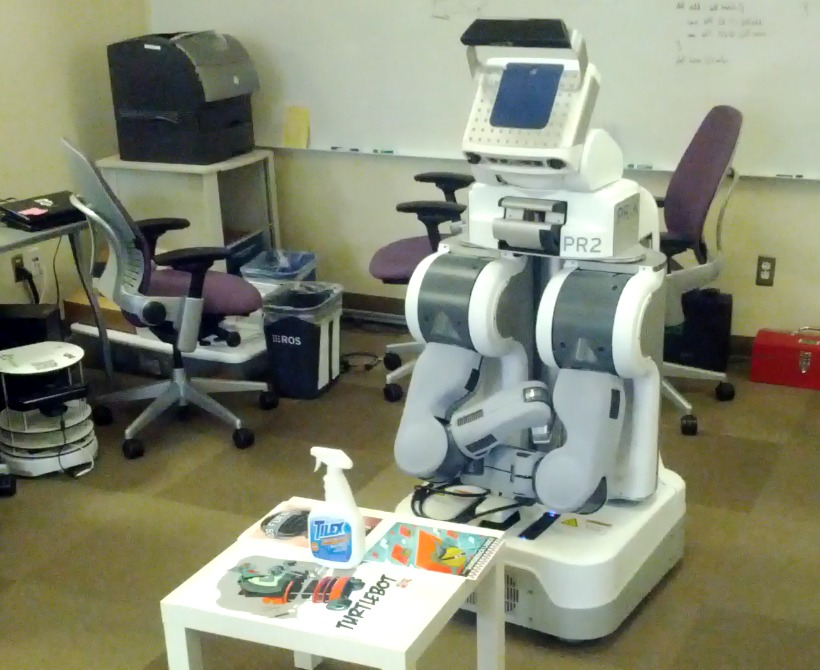
\includegraphics[width=\linewidth]{../tizer/pr2.jpg}
                \caption{PR2 moving around a fixed table}                
        \end{subfigure}%                 
        \end{center}
        
        \begin{subfigure}[b]{0.49\linewidth}
                \centering
                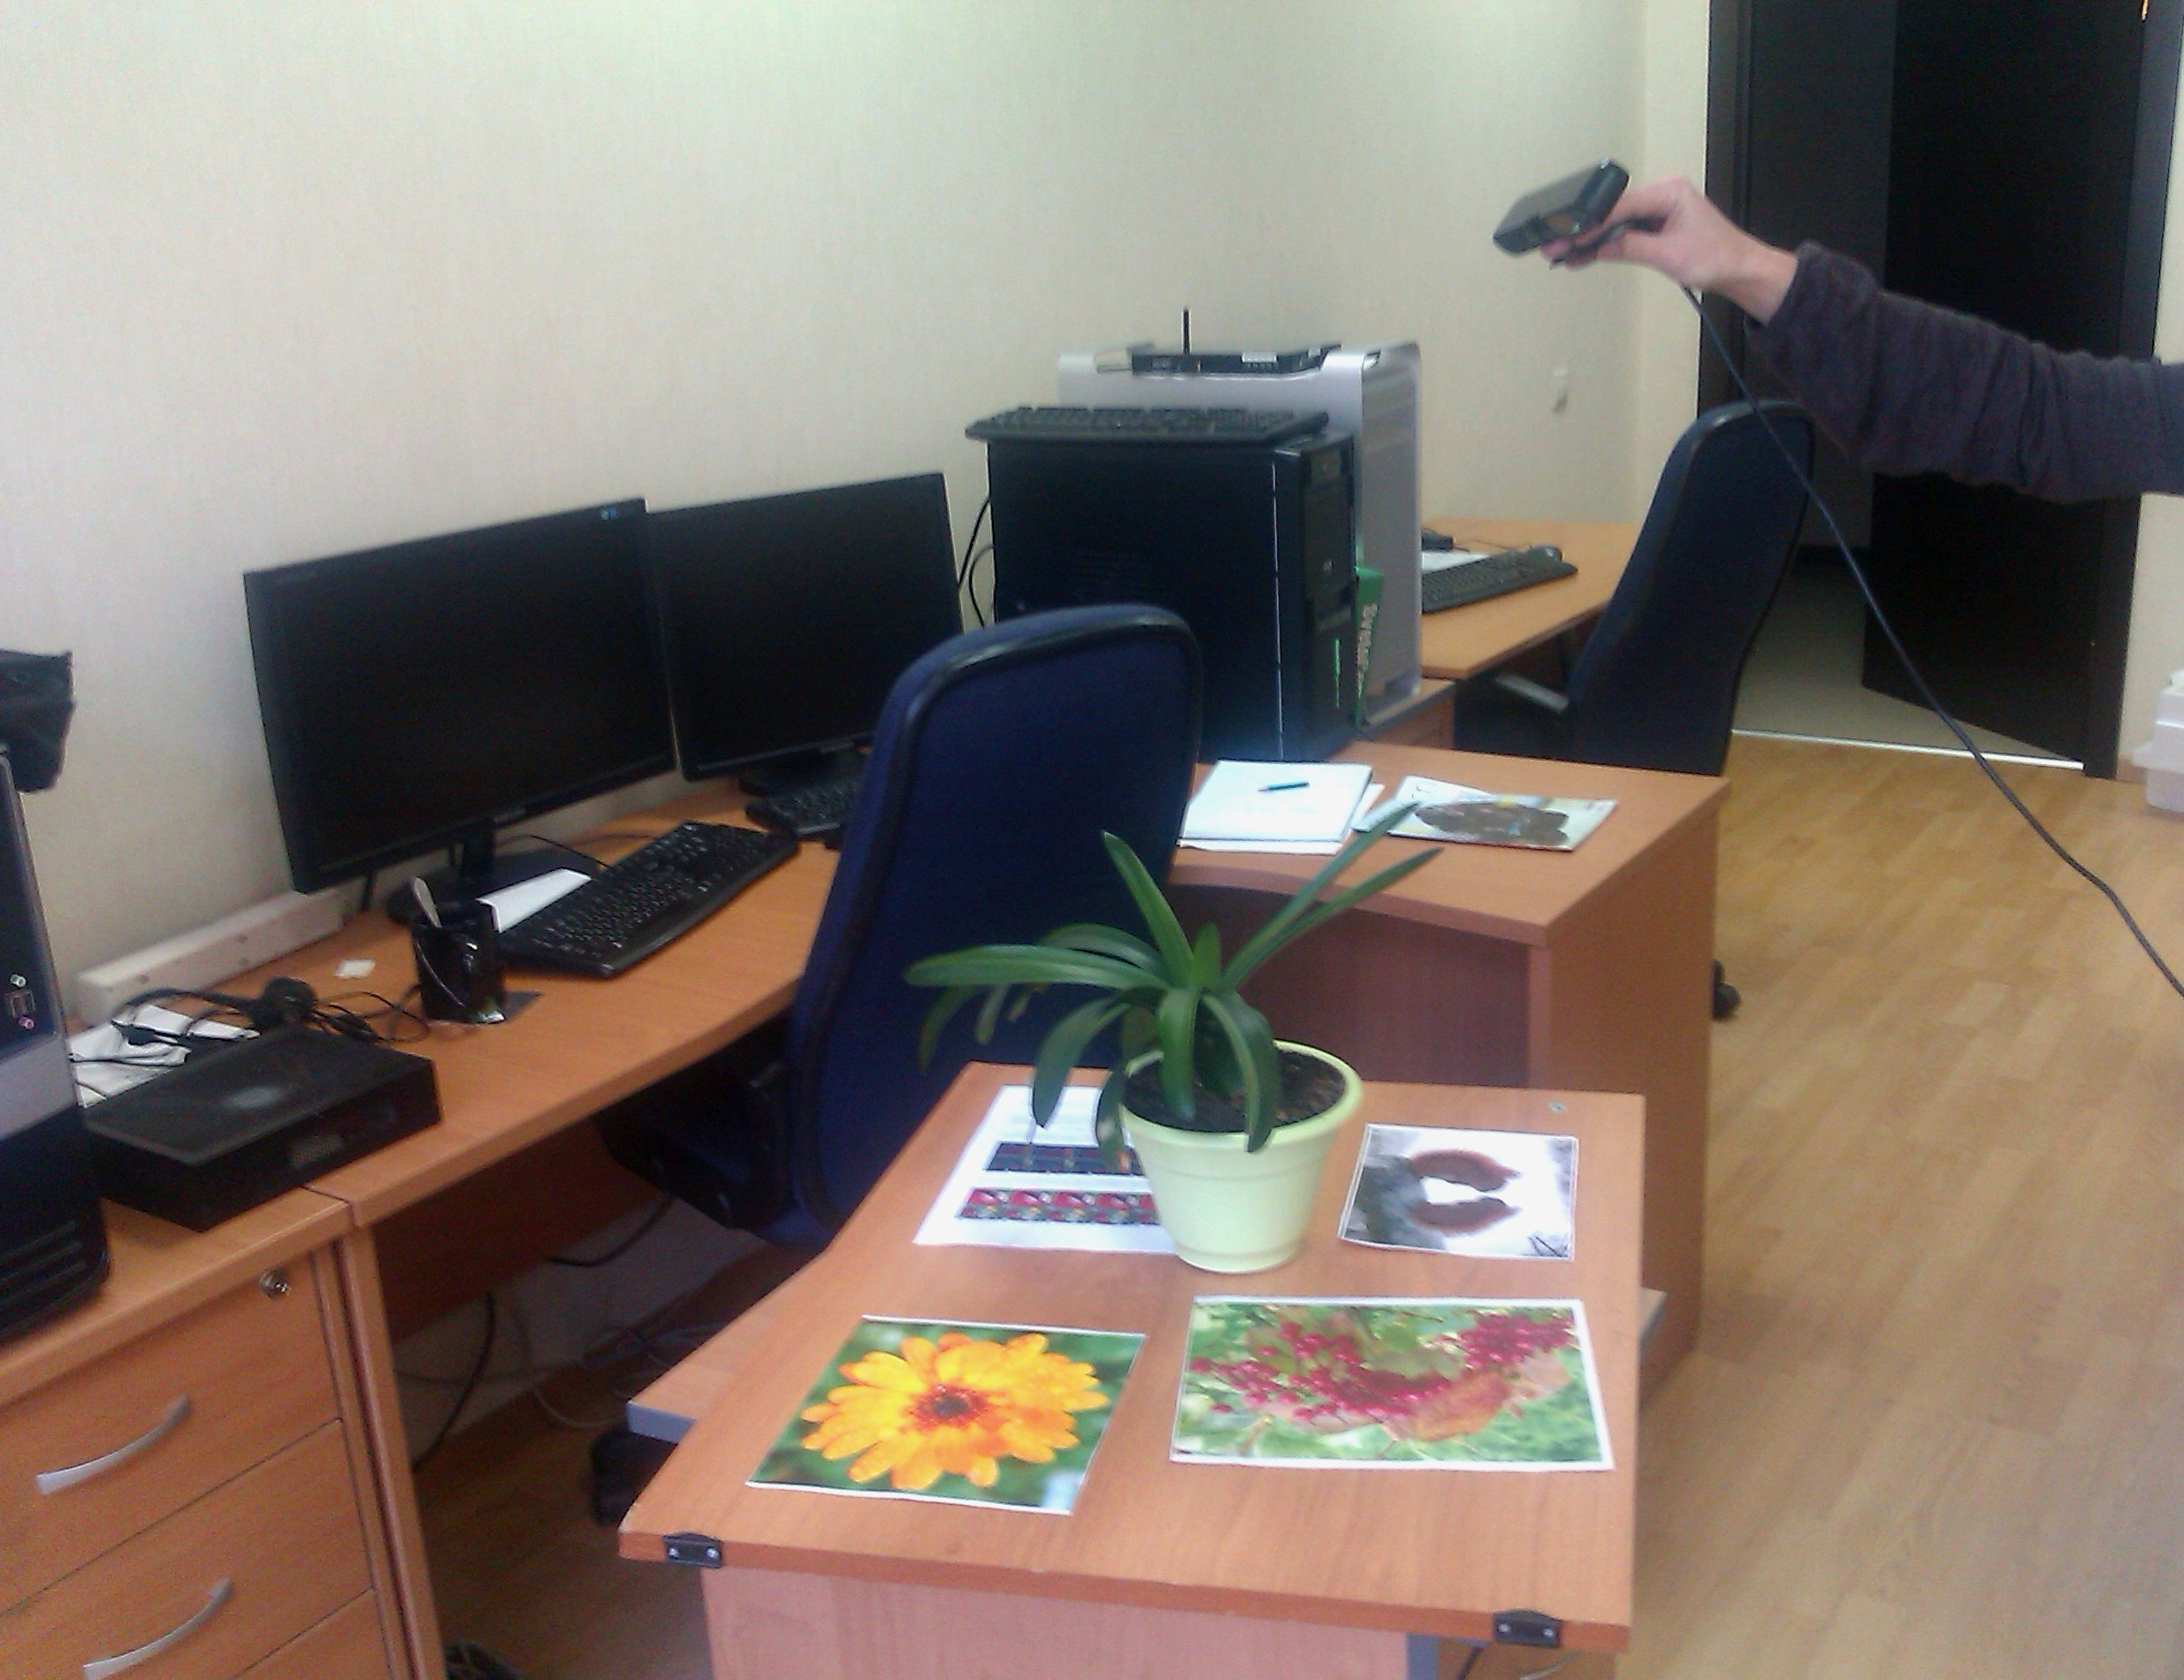
\includegraphics[width=\linewidth]{../tizer/handHeld.jpg}
                \caption{Hand-held sensor moving around a fixed table}
        \end{subfigure}%
        ~ %add desired spacing between images, e. g. ~, \quad, \qquad etc.
          %(or a blank line to force the subfigure onto a new line)
        \begin{subfigure}[b]{0.49\linewidth}
                \centering
                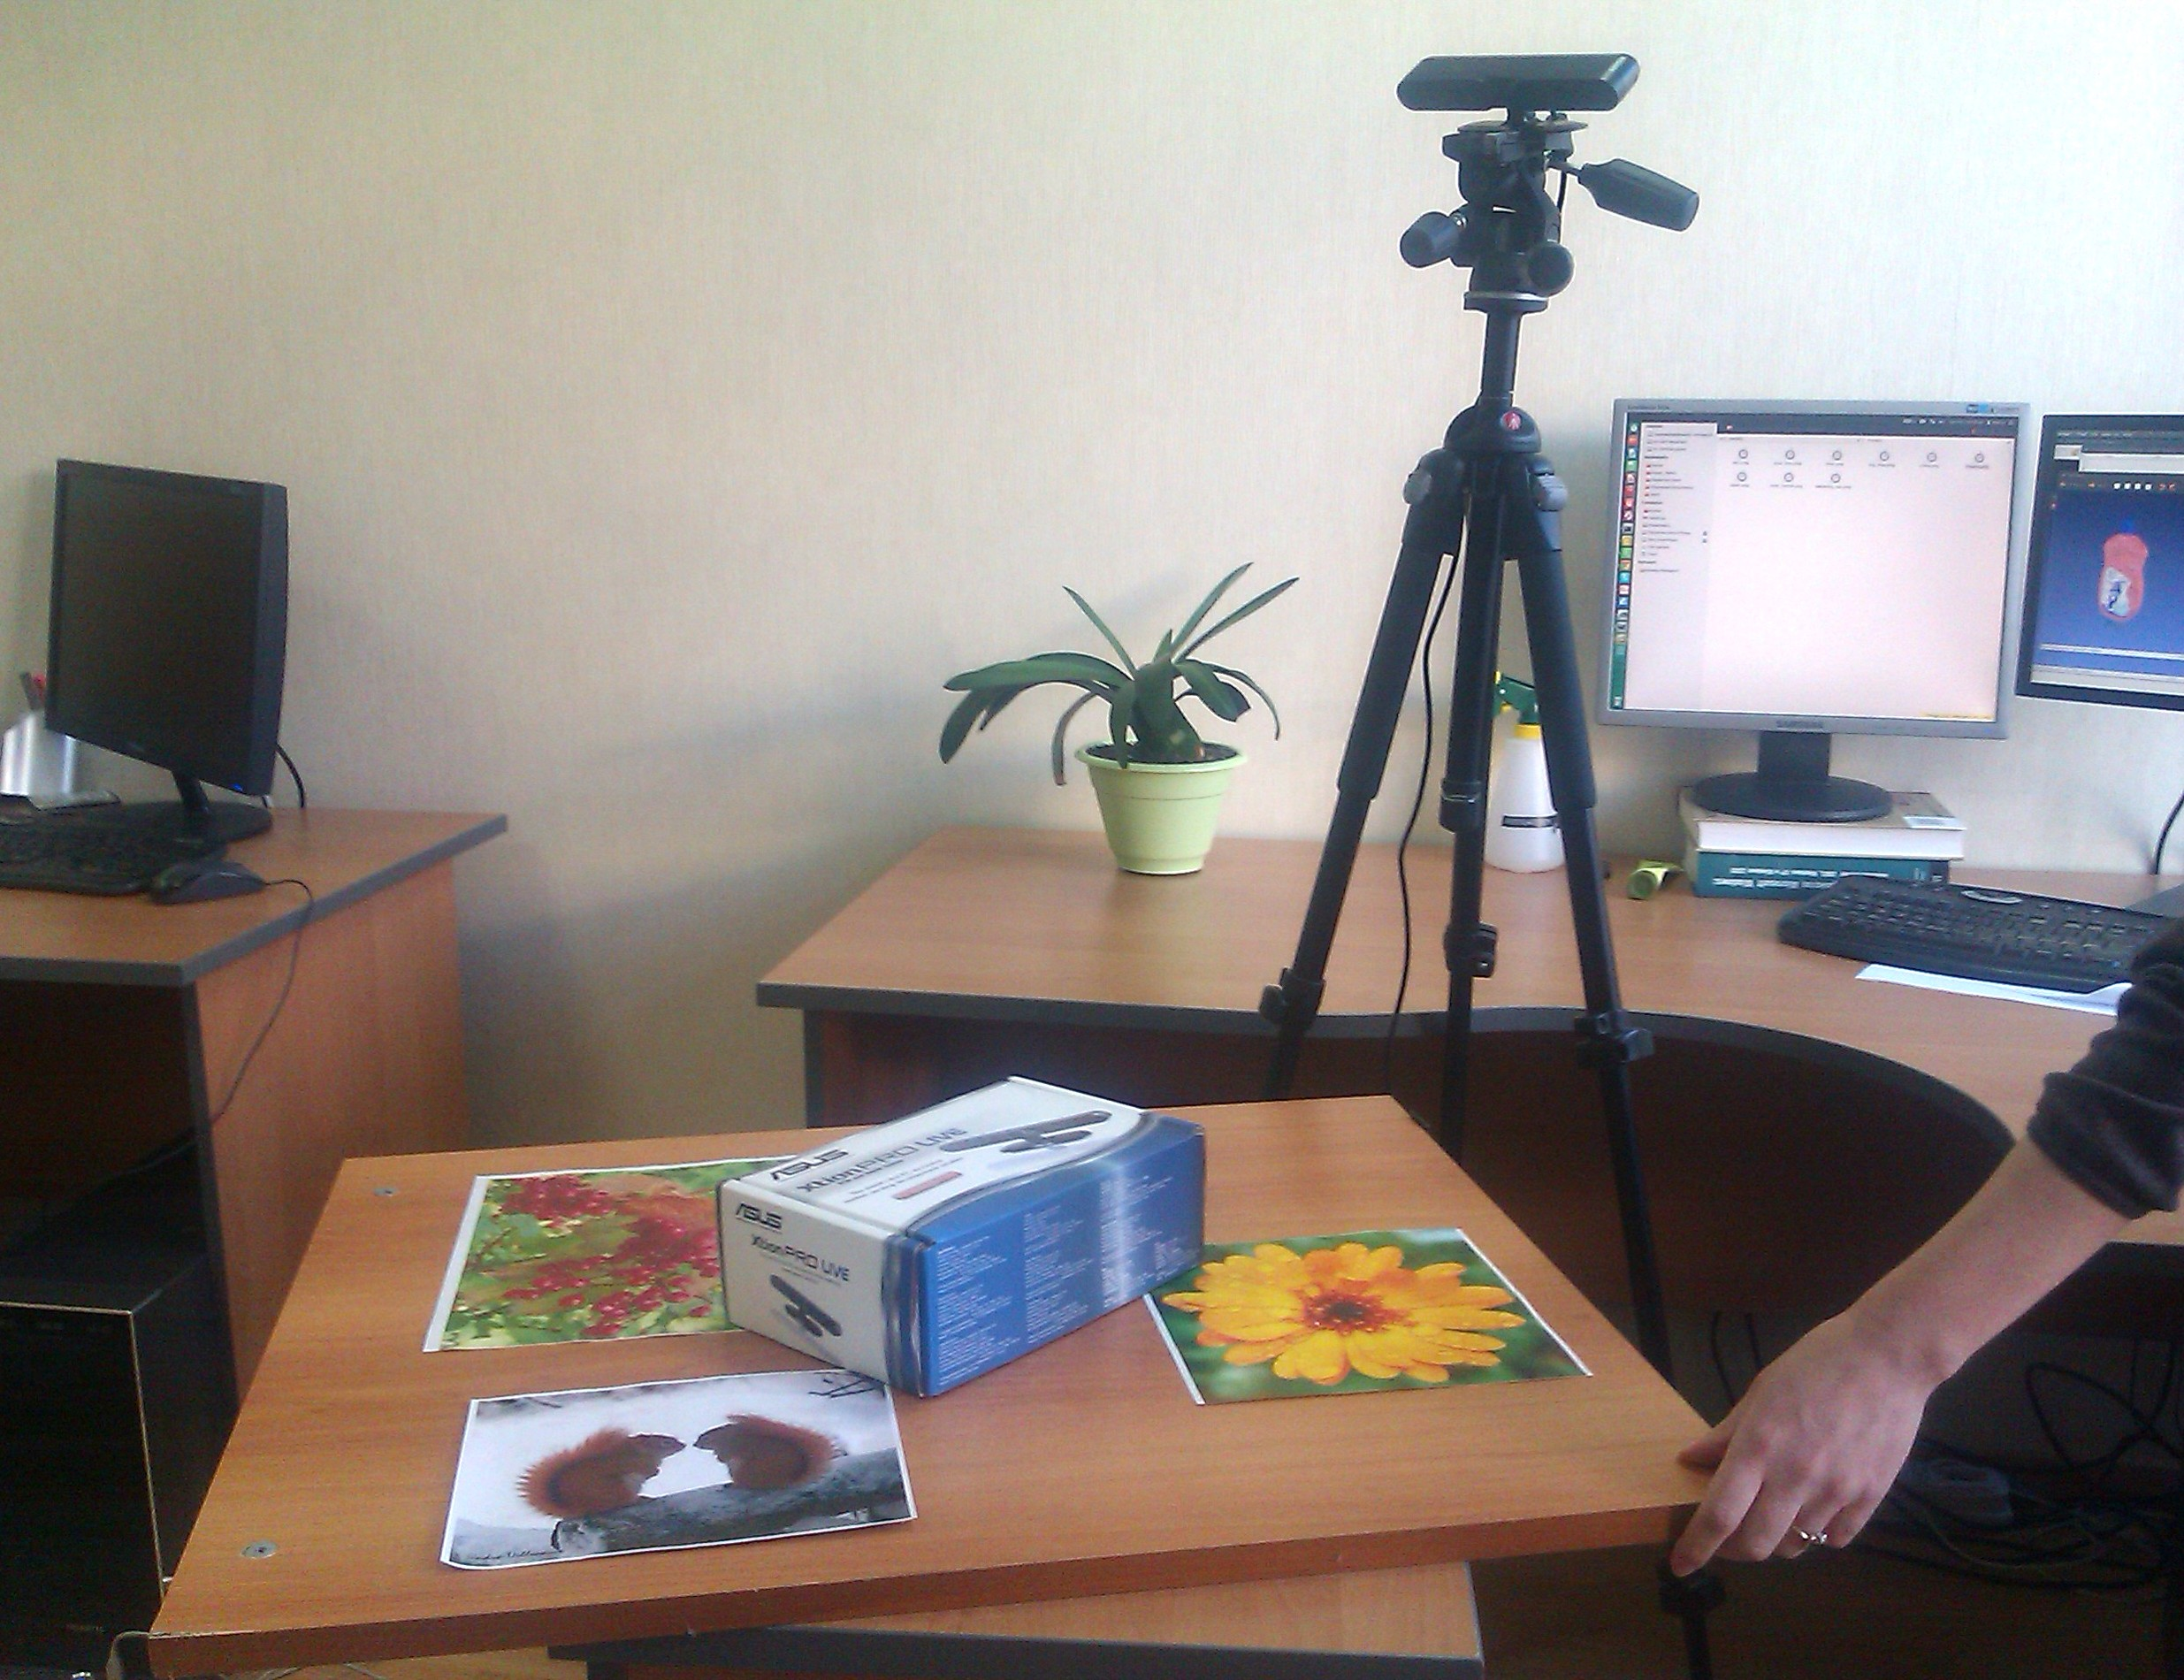
\includegraphics[width=\linewidth]{../tizer/turntable.jpg}
                \caption{Turning table in front of a fixed sensor}
        \end{subfigure}
        
        \begin{subfigure}[b]{\linewidth}
                \centering
                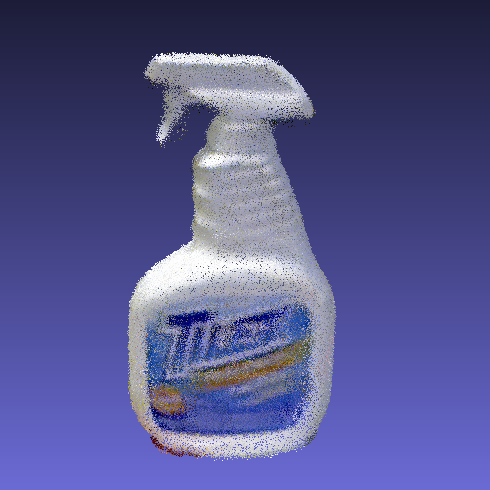
\includegraphics[width=0.49\linewidth]{../tizer/tilexFrontal.png}
%                \caption{Segmentation}
%        \end{subfigure}%
%        ~ %add desired spacing between images, e. g. ~, \quad, \qquad etc.
%          %(or a blank line to force the subfigure onto a new line)
%        \begin{subfigure}[b]{0.49\linewidth}
%                \centering
                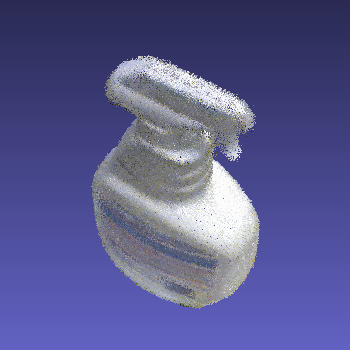
\includegraphics[width=0.49\linewidth]{../tizer/tilexTop.png}
                \caption{A model of "Tilex" bottle captured by PR2}
        \end{subfigure}
        \caption{Examples of the algorithm working: (a)-(c) are the supported 
        capturing setups, (d) results of working}
        \label{fig:tizer}
\end{figure}


Probably the most common tabletop object scanning setup in computer 
%TODO: ref, proof
vision or robotics laboratories is a table or a turntable with
visual markers on it (e.g. chessboards) which
are used for the camera pose estimation and can be applied for 
an object segmentation too. \cite{ectoObjectRecognitionCapture} also 
provides an option to replace special visual markers by arbitrary texture. 
But in this case there is a training stage for textured visual features:
the user has to capture a canonical image of the empty table from
a planar frontal view before scanning. Preparing the markers
and a training stage for texture are inconvenient for a person and
hard or impossible for a robot. 

Our approach also requires arbitrary
texture on a table at our scanning setup. For the camera motion estimation 
we use state-of-the-art dense RGB-D odometry algorithm \cite{steinbrucker2011real} 
instead of feature-based tracking 
and it allows us to eliminate a training stage.
We can not abandon the requirement of texture because the depth-based
techniques for the camera motion estimation like ICP \cite{besl1992method} 
are not reliable in scenes with the dominant plane \cite{rusinkiewicz2001efficient} which we have.


For the same reason
the impressive technique KinectFusion \cite{newcombe2011kinectfusion} 
which uses ICP for camera poses estimation can not be applied in our capturing setup.
Usage of KinectFusion without a table plane or intentionally cluttered table 
returns to the problem of automatic object segmentation.
Also KinectFusion smooths captured surfaces too much, \cite{meister2012when} measured that
the system can resolve object details with a minimum size of approximately 10mm.
% TODO "measured that the system can resolve object details with a minimum size of approximately 10mm" is a copy-paste 
% from the cited paper

The other recent approach \cite{stuckler2012model} for 3D model learning 
exploits both RGB and depth information of an input frame to estimate a camera pose 
in relation to an aggregated scene model represented by the multi-resolution surfels map.
Using RGB data can allow this method to get stable pose estimation
for scenes with a dominant plane. Also camera pose estimation in "frame-to-model" mode
in this work as well as in KinectFusion leads to less accumulation of the pose estimation error. 
But it is still possible that there are small camera pose errors which result in
small misalignment of RGB-D scans. Our approach applies global alignment of scans
to increase their consistency to the input RGB and depth data.

Model reconstruction can be referred to the problem of simultaneous localization
and mapping (SLAM). There are a lot of SLAM approaches including those ones working
with RGB-D cameras, e.g. \cite{stuckler2012integrating},
\cite{endres2012evaluation}, \cite{henry2012rgb}, \cite{strasdat2011double}. But in contrast to our goal,
a scanning relatively small objects, such approaches are more oriented for
a more long-lasting navigation and large space mapping. Many of them aim at
real-time working on a robot, so they can afford alignment of scans 
as rigid-bodies only. 
The recent work \cite{ruhnke2012highly} introduced a post-processing procedure for the output of SLAM systems
which considers the registered scans as non-rigid bodies and produces highly accurate
surface of a model by simultaneous refinement of model points positions and camera poses.
Pairwise and global alignment of camera poses and depth maps which includes non-rigid 
deformations is also applied in \cite{cui2012algorithms}. Their results include tests on the Kinect
sensor data but their work is mainly oriented for Time-of-Flight (ToF) cameras. Considering non-rigid deformations 
of depth maps allowed them to get high quality 3D models even for very noisy ToF depth measurements.
So we also follow the idea of simultaneous optimization of camera poses and model points 
for the final non-rigid refinement. We exploit the knowledge 
about the supported scanning setup and both RGB and depth 
data to produce initial alignment of scans as rigid bodies
and then refine it by such optimization non-rigidly.

In this paper we provide a complete pipeline for object scanning
in the tabletop capturing setup. This setup has natural requirements
about a table and texture for the stable camera pose estimation,
coping with symmetric objects and automatic object segmentation, and it is general enough
to use it by a person or a robot. A base of 42 objects was
scanned successfully by a PR2 robot, a person with a hand-held camera 
and using a turntable (see examples of scanning setups 
in Fig.~\ref{fig:tizer}).


\section{OVERVIEW OF THE SCANNING PIPELINE}

The goal of our scanning pipeline is to produce an accurate 3D model
of an object captured by a person or a robot.
In order to achieve this goal, we
impose restrictions on a scanning setup and process: it should be
one turn of an RGB-D camera around a textured table with an object. 

A textured table allows solving the following problems:

\begin{itemize}

\item \textit{Automatic object segmentation}. It is easy to find the table plane
in a scene and segment an object placed on the table using RGB-D data.
\item \textit{Stable camera pose estimation}. Due to presence of texture
a state-of-the-art RGB-D visual odometry algorithm can be applied.
Alternative dense visual odometry methods based only on depth measurements
like ICP are not reliable in a scene with a prevalent plane \cite{rusinkiewicz2002real}
because such algorithms need rich 3D structures for registration but a plane is too homogeneous
(it is like trying to match textureless objects by looking for textured 2D features).
Both dense approaches
suppose a static scene and they can tolerate only slight movements in the scene.
So to obtain a stable camera motion estimation we run the odometry using only
%TODO: replace "can be considered static" with "are static"
points of a table and an object because they can be considered static.
It allows applying the algorithm in dynamic scenes where there are moving objects e.g. people, pets or robots.
\item \textit{Scanning symmetric textureless objects}. Registration of scans of such an object
is most likely to fail if it uses object points only. So an object pose should be known beforehand like in \cite{krainin2011manipulator}
or some part of a scene with
texture or 3D features should also be used to add sufficient constraints.
Textured table is exploited for this purpose in our pipeline
and so the algorithm is able to create models of symmetric textureless objects.
\end{itemize}

%TODO: put somewhere?
%We require the full turn
%to get a loop closure in a trajectory which is used to compensate a drift
%of an odometry.

One turn around the table simplifies loop closure detection and poses graph construction
in contrast to an arbitrary camera trajectory
and so makes the algorithm more robust because setting incorrect associations
in the graph can lead to catastrophic implications in the offline graph
optimization \cite{sunderhauf2012switchable}.
However, a complex object may require a more complicated trajectory
or merging several scans together to capture all parts of the object %TODO: ref
and this is a direction for future work.

Our pipeline consists of online and offline stages. The online part is the capture of RGB-D data,
initial estimation of camera poses using frame-to-frame odometry,
selection of keyframes set, detection of loop closure. The offline part is aimed for
the global refinement of camera poses and model points. There are three stages
of the offline refinement:

\begin{enumerate}
\item At first we seek the configuration of camera poses that is
maximally consistent to the pure odometry estimations without 
considering the RGB-D frames data. The input camera poses of this stage
are estimated by frame-to-frame odometry and this produces drift: 
the farther a camera pose is from the starting position of the trajectory, 
the larger an error of its estimation becomes. The drift is compensated
by applying the constraint from the detected loop closure 
that redistributes the accumulated error among the poses evenly.

\item Then we refine the camera poses to achieve 
consistency of corresponding RGB-D scans as rigid bodies.

\item The last stage is mainly for the refinement of model points. It uses the idea similar to \cite{ruhnke2012highly}
that considers individual scans as non-rigid bodies and optimizes
model points and camera poses simultaneously to achieve highly accurate alignment.

\end{enumerate}

\section{ONLINE STAGE}

This stage is performed during the capture of RGB-D data. It includes
frame-to-frame estimation of camera poses, selection of keyframes and 
detection of loop closure.

We use the dense RGB-D visual odometry
method \cite{steinbrucker2011real} for the camera motion estimation.
It is accurate and fast enough to apply it online
(execution time of 12.5Hz is reported in \cite{steinbrucker2011real}
on a single Intel Xeon E5520 CPU).
Our open-source implementation\footnote{\label{note1}\href{http://bit.ly/rgbd\_module}{http://bit.ly/rgbd\_module}} of this algorithm
introduces optimization which allows it to work at 23Hz on one core
of Intel Core i5 without using SSE.
It is achieved by using only points with high gradient in the target intensity image
to compute odometry (the same idea was proposed in \cite{tykkala2011direct} for another odometry algorithm).
Other points provide less information for alignment
and so they can be ignored without loss in accuracy of the RGB-D odometry algorithm
as we checked using the TUM RGB-D benchmark \cite{sturm12iros}.
% TODO prove it? it's easy to provide results on TUM, but this in not our main goal.  

The RGB-D odometry method assumes absence of motion in a scene and it is not
robust to large movement in the scene. So to satisfy this requirement
and keep stability of the odometry we run it only
on the points of a table and an object. The mask of table points
is found in real-time using an approach from \cite{poppinga2008fast}. An object mask is
obtained by extracting points in a virtual 3D prism above the table \cite{rusu2009detecting}.
Using only the points
of a table and an object in the camera pose estimation brings one more advantage:
moving a camera around a fixed table becomes equivalent to rotating
a table in front of a fixed camera. So our system covers a scanning setup with a turntable too
and we provide experiments both with a hand-held sensor and a turntable.

It is still possible to get an incorrect pose from RGB-D odometry
because of light changes and motion blur from hand jitter.
We filter out such outliers:

\begin{enumerate}
 \item If a returned transformation between two frames is beyond the basin of convergence
 of the RGB-D odometry (about 15cm and 15 degrees in our experiments) most likely it is an outlier.
 \item We also wrap a source frame using an estimated transformation,
 compute the difference between target and warped frames 
 and filter the transformation out if
 depth and intensity differences are large for many pixels.
\end{enumerate}

%TODO: is there a backward search for a valid transformation?
A pose of each new frame is estimated relatively to the last frame
with a valid transformation from the odometry.

%TODO: need more details
A keyframes set is selected during the capture.
The used criterion is translation and rotation thresholds 
between a current frame and the last keyframe.

The frame-to-frame estimation of camera poses from the RGB-D 
odometry results in drift. It is usually not too large in our case
due to high accuracy of the used odometry method \cite{steinbrucker2011real}
and only one turn around a table.
But it still should be compensated and the loop closure event is detected to solve this problem.
%TODO: how much is "large enough"?
When length of the trajectory is large enough, we begin to estimate the
odometry transformation between each current frame and the starting one. 
If the returned transformation passes through the described filters, 
this means the current pose is close to the first one and 
the trajectory has been closed. When the loop closure is detected 
the capture is stopped.

Thus each frame is passed through the steps:

\begin{enumerate}
 \item plane and object segmentation,
 \item odometry estimation and outliers filtering,
 \item the check: is it a keyframe?
 \item the check: is it loop closure?
\end{enumerate}

We also should note that loop closure detection using the RGB-D odometry requires
the last pose of a camera to be in a basin of
the algorithm convergence (about 15cm and 15 degrees) from the first pose. 
To allow a larger difference between the first and the last frames
another approach can be used in detection of loop closure, e.g.
an often used method of matching visual features, like
SIFT \cite{lowe2004distinctive}, SURF \cite{bay2006surf}, ORB \cite{rublee2011orb}.
However, these feature detectors and descriptors failed to match even
relatively close frames in our capturing setup of turning around a textured table.
The reason is large affine distortions
and these standard features are not fully affine invariant.
ASIFT \cite{morel2009asift} was able to overcome this problem
and perfectly coped with the task in our experiments,
however, it has to be strongly optimized before its usage in an online application.

The output of the online part is a set of consecutive keyframes with 
estimated poses and the transformation between the first and the last 
keyframes from loop closure.


\section{OFFLINE STAGE}

The purpose of the offline processing is refinement of the online-estimated 
camera poses as well as points of scans to get a model maximally 
consistent with the captured RGB-D data. We achieve this in three steps by 
solving least squares optimization problems. The cost function is extended at each step 
by introducing additional terms which can be reliably computed
thanks to refinement from a previous stage.

%TODO is it clear that constrains are the same but they are with new data (new corresps, etc.)?

The input of the offline stage is a set of initial camera poses $\{x_n^{(0)},~n=1,\dots, N\}$ 
estimated by accumulating consecutive frame-to-frame odometry transformations 
$\{z_n,~n=1,\dots, N-1\}$  
(where $z_n$ is the odometry transformation from the frame $n+1$ to the frame $n$)
%from each 
%current frame to the previous one
and loop closure constraint $z_{N}$, 
i.e. odometry transformation from the last frame to the first one.

\begin{figure}[t]
	\centering
        \begin{subfigure}[b]{0.45\linewidth}
                \centering
                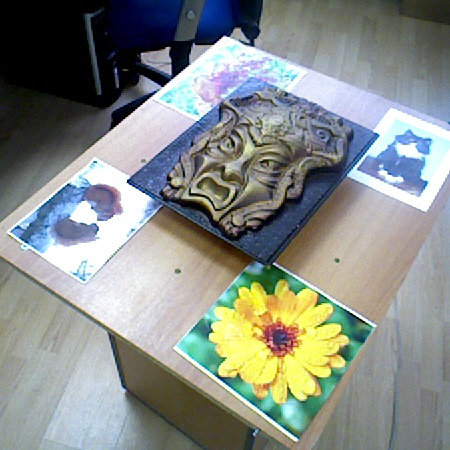
\includegraphics[width=\linewidth]{../models/gorgon_train.jpg}
                \caption{}
        \end{subfigure}%
        ~ %add desired spacing between images, e. g. ~, \quad, \qquad etc.
          %(or a blank line to force the subfigure onto a new line)
        \begin{subfigure}[b]{0.45\linewidth}
                \centering
                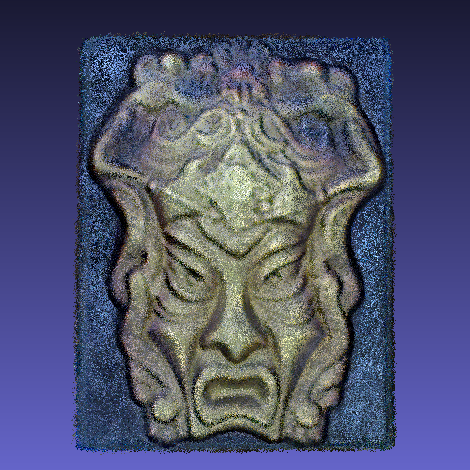
\includegraphics[width=\linewidth]{../models/gorgon_color_model.png}
                \caption{}
        \end{subfigure}

        \centering
        \begin{subfigure}[b]{0.45\linewidth}
                \centering
                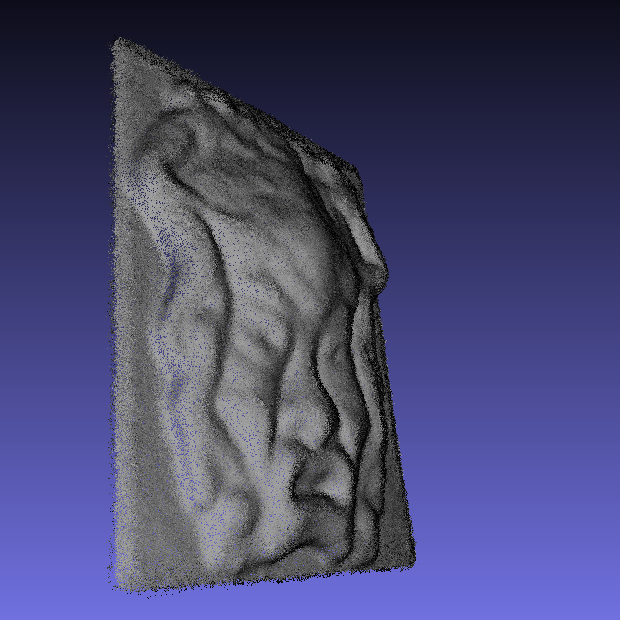
\includegraphics[width=\linewidth]{../models/gorgon_gray_model1.png}
                \caption{}
        \end{subfigure}%
        ~ %add desired spacing between images, e. g. ~, \quad, \qquad etc.
          %(or a blank line to force the subfigure onto a new line)
        \begin{subfigure}[b]{0.45\linewidth}
                \centering
                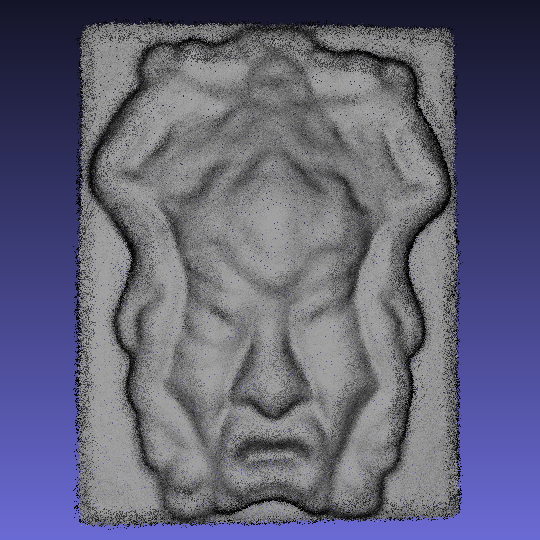
\includegraphics[width=\linewidth]{../models/gorgon_gray_model.png}
                \caption{}
        \end{subfigure}
        \caption{Scanning the relief picture of Gorgon: (a) train image example,
        (b) colored model (point cloud), (c,d) uncolored point cloud}
        \label{fig:gorgon}
\end{figure}

At the first step we compensate the drift in frame-to-frame estimated camera poses and 
make them consistent to the odometry constrains (including the transformation from the last pose
to the first one) by minimizing the following cost function
with regard to camera poses $x_{1:N}$:
\begin{equation} \label{eq:ffirst}
F_{SE3}(x_{1:N}) = \sum_n (z_n \ominus y_n)^T \Omega_{SE3} (z_n \ominus y_n),
\end{equation}
where $\ominus$ is the inverse compounding operator \cite{lu1997globally},
$y_n=x_{n+1} \ominus x_{n}$ ($n=1,\dots, N-1$), $y_N=x_N \ominus x_1$,
the matrix $\Omega_{SE3}$ is an information matrix that weighs an odometry uncertainty \cite{kuemmerle2011g2o}.

The first step does not use directly RGB-D information of the frames and they are
still slightly misaligned. So an RGB-D term is added to refine the camera poses at the second step 
to achieve better consistency among all RGB-D scans.
The first step improved accuracy of poses by exploiting the loop closure event.
So corresponding points between two frames can be found now by using
the fast projective data association algorithm \cite{rusinkiewicz2001efficient}.
Two kinds of terms are added for each pair of corresponding 3D points of each frames pair
to minimize their 3D distances and intensity difference.

We use a common notation: $p_{nk}$ denotes $k^{th}$ 3D point of 
the $n^{th}$ frame. So the cost function responsible for the shape consistency is
a sum of the ICP odometry terms:
\begin{equation} \label{eq:ficp}
    F_{ICP}(x_{1:N}) = \sum_{n,m,i,j} \Delta p_{nmij}^T \Omega_{mj} \Delta p_{nmij},
\end{equation}
\begin{equation}
    \Delta p_{nmij}=(p_{ni} \oplus x_n) \ominus x_m - p_{mj},
\end{equation}
where summation is done over all corresponding points and $\Omega_{mj}$ is 
an information matrix that results in the point-to-plane 
distances in \eqref{eq:ficp}.

\begin{figure}[t]
	\centering
        \begin{subfigure}[b]{0.45\linewidth}
                \centering
                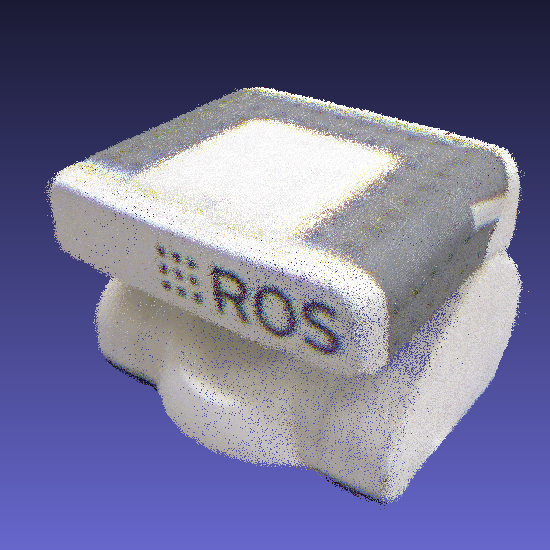
\includegraphics[width=\linewidth]{../models/pr2_full.png}
                \caption{}
        \end{subfigure}%
        ~ %add desired spacing between images, e. g. ~, \quad, \qquad etc.
          %(or a blank line to force the subfigure onto a new line)
        \begin{subfigure}[b]{0.45\linewidth}
                \centering
                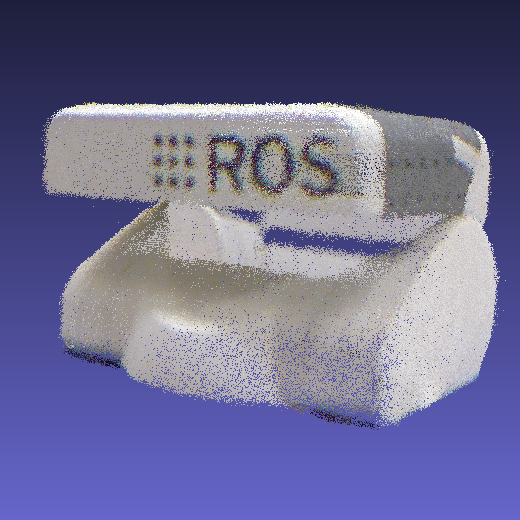
\includegraphics[width=\linewidth]{../models/pr2_holes.png}
                \caption{}
        \end{subfigure}
        \caption{Example of the problem with holes in a model point cloud 
        due to occlusions of object parts:
        (a) view of PR2 head model close to one a camera had while capturing,
        (b) view that is lower a camera trajectory: there is a hole under 
        the top part of the head}
        \label{fig:pr2}
\end{figure}

The cost function responsible for the intensity consistency is
a sum of the RGB-D odometry terms:
\begin{multline} \label{eq:frgbd}
F_{RGBD}(x_{1:N}) = \\
= \omega_{rgbd} \sum_{n,m,i} \biggl[I_n(\pi p_{ni}) - I_m\Bigl(\pi \bigl((p_{ni} \oplus x_n) \ominus x_m\bigr)\Bigr) \biggr]^2,
\end{multline}
where $I_n$ is an intensity image, $\pi$ is an image projection function, $\omega_{rgbd}$
is a weight of the RGB-D term.

So the following function is minimized at the second step:
\begin{equation} \label{eq:fsecond}
F_{SE3}(x_{1:N}) + F_{ICP}(x_{1:N}) + F_{RGBD}(x_{1:N}).
\end{equation}

In order to increase basin of convergence 
we minimize \eqref{eq:fsecond} using a coarse-to-fine scheme 
what visual odometry algorithms often do. 
We recompute correspondences between frames
after each iteration of each pyramid level.

The optimization of the function \eqref{eq:fsecond} is run 
twice for different points. The first time the points of a table and an object are used  because 
the textured table points give necessary constrains in the case of symmetric and textureless object.
The second time \eqref{eq:fsecond} is minimized using only object points to refine 
camera poses relatively to interesting parts of scans only.

We get accurate camera poses and scans aligned properly 
as rigid bodies after the second step. But there is camera noise in depth measurements and small 
misalignment of scans due to it. The third step produces a final accurate model by
simultaneous optimization of object points coordinates and camera poses.

This step exploits the idea of \cite{ruhnke2012highly} but our version 
is simplified due to previous steps: 

\begin{itemize}
 \item As we already have well-aligned scans at this stage, we can apply 
 the fast projective algorithm \cite{rusinkiewicz2001efficient} 
 (with filtering by differences in depth values, 
 normals and intensity) to find correspondences instead of slower
 normal-shooting which \cite{ruhnke2012highly} uses.
 \item We consider that each object 3D point of each frame is 
 a surfel centered in this point i.e. for each frame there are as many 
 surfels as object pixels it has. We don't aim for large space model refinement as \cite{ruhnke2012highly}
 so it is not necessary for us to use a more compact scan surface representation by covering several pixels 
 by one surfel.
 \item After the surfel 3D position was refined we update only depth value 
 in the original pixel of a frame depth map. This conforms with the purpose to 
 refine noisy depth measurements using information from other scans.
\end{itemize}

With these remarks the error function for the surfel positions refinement 
$F_{model}(x_{1:N}, M)$ (where $M$ is a set of 3D points from 
all frames) in our approach is the same as formula (11) in \cite{ruhnke2012highly}.

So the following function is minimized at the third step:
\begin{multline} \label{eq:fthird}
F_{SE3}(x_{1:N}) + F_{ICP}(x_{1:N}) + F_{RGBD}(x_{1:N}) + \\
+ F_{model}(x_{1:N}, M).
\end{multline}

After \eqref{eq:fthird} was minimized we filter out the points 
which don't have correspondences or have a small number of correspondences in
all other frames because they were not refined or the refinement result
is doubtful due to small number of used correspondences.

In order to solve the least squares optimization problems 
of the three steps \eqref{eq:ffirst}, \eqref{eq:fsecond} and \eqref{eq:fthird} 
they were formulated as the graph-based optimization tasks.
These tasks were solved by applying the efficient g2o framework 
\cite{kuemmerle2011g2o} which exploits sparseness of the graph structure.

The output of the offline stage is the final model representing
a colored point cloud where the color of each 3D point is taken 
by its pixel coordinates from the frame where the point was originaly 
captured (see an example in Fig.~\ref{fig:gorgon}).

\begin{figure}[th]
        %\begin{center}
	\centering
        \begin{subfigure}[b]{0.5\linewidth}
                \centering
                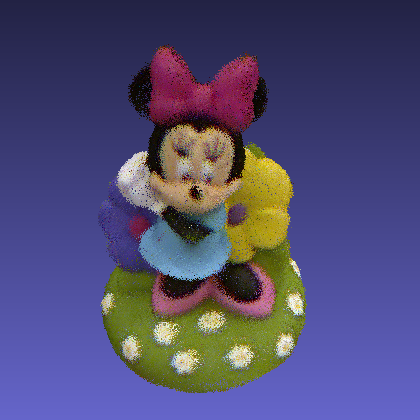
\includegraphics[width=\linewidth]{../models/mouse.png}
                %\caption{PR2 moving around a fixed table}                
        \end{subfigure}%                 
        %\end{center}
        \begin{subfigure}[b]{0.5\linewidth}
                \centering
                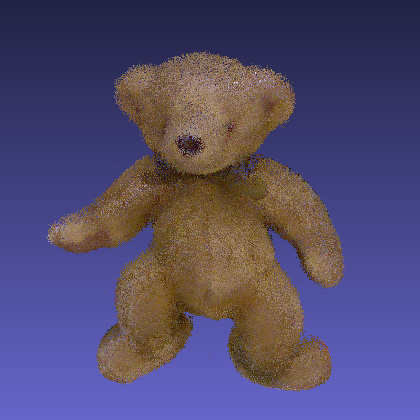
\includegraphics[width=\linewidth]{../models/bear.png}
                %\caption{Hand-held sensor moving around a fixed table}
        \end{subfigure}
        
        
        \begin{subfigure}[b]{0.5\linewidth}
                \centering
                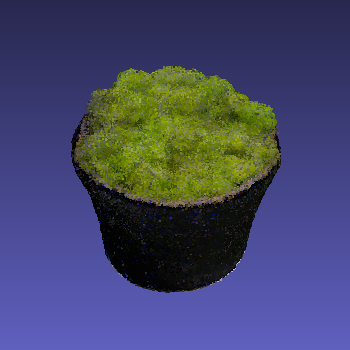
\includegraphics[width=\linewidth]{../models/plant.png}
                %\caption{Turned table beyond a fixed sensor}
        \end{subfigure}%
        \begin{subfigure}[b]{0.5\linewidth}
                \centering
                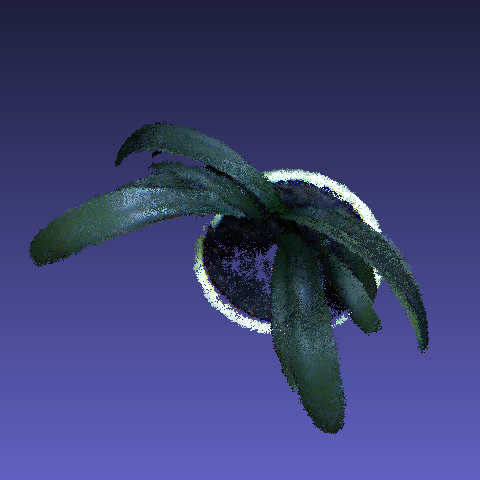
\includegraphics[width=\linewidth]{../models/clivia.png}
                %\caption{Turned table beyond a fixed sensor}
        \end{subfigure}
        
        \begin{subfigure}[b]{0.333333\linewidth}
                \centering
                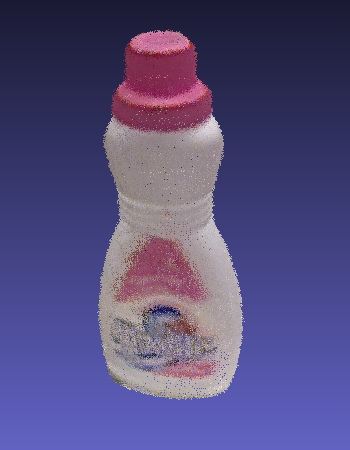
\includegraphics[width=\linewidth]{../models/rose_bottle.png}
                %\caption{Turned table beyond a fixed sensor}
        \end{subfigure}%
        \begin{subfigure}[b]{0.333333\linewidth}
                \centering
                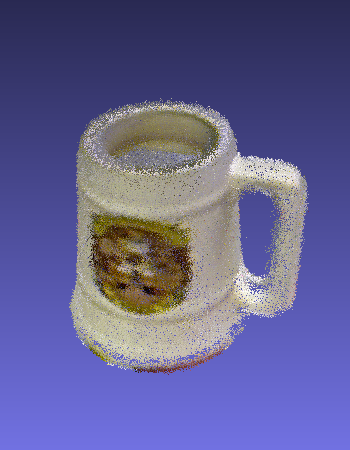
\includegraphics[width=\linewidth]{../models/big_mug.png}
                %\caption{Turned table beyond a fixed sensor}
        \end{subfigure}%
        \begin{subfigure}[b]{0.3333\linewidth}
                \centering
                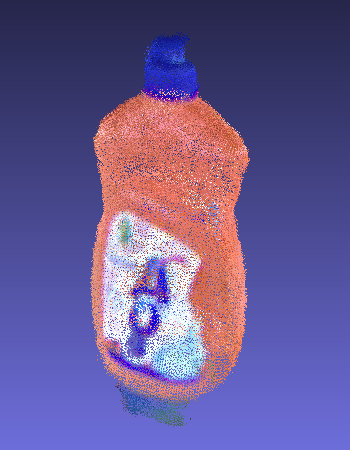
\includegraphics[width=\linewidth]{../models/aos.png}
                %\caption{Turned table beyond a fixed sensor}
        \end{subfigure}
        
        \begin{subfigure}[b]{0.5\linewidth}
                \centering
                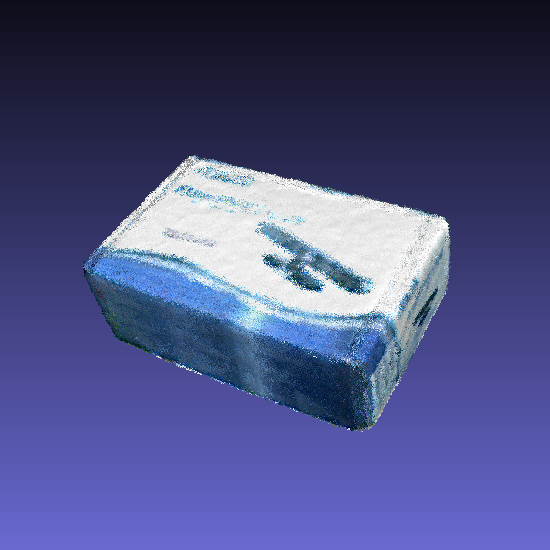
\includegraphics[width=\linewidth]{../models/asus_box.png}
                %\caption{Turned table beyond a fixed sensor}
        \end{subfigure}%
        \begin{subfigure}[b]{0.5\linewidth}
                \centering
                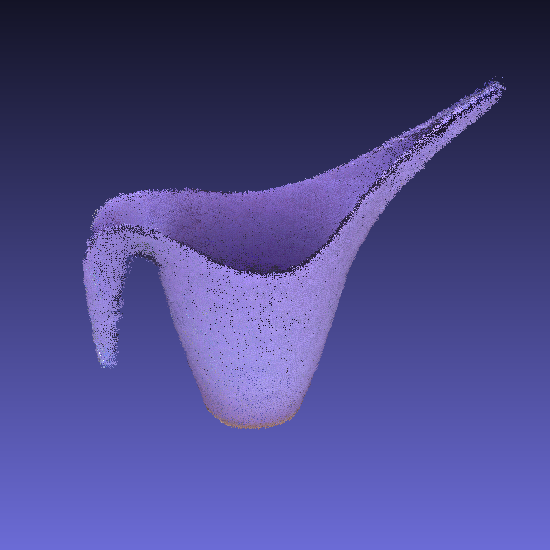
\includegraphics[width=\linewidth]{../models/watering_can.png}
                %\caption{Turned table beyond a fixed sensor}
        \end{subfigure}
        \caption{Examples of reconstructed models}
        \label{fig:results}
\end{figure}

\section{RESULTS}
 
The presented system was tested in three capturing scenarios:

\begin{itemize}
 \item A person with a hand-held camera captured an object placed on a fixed table.
 \item A PR2 robot with its RGB-D sensor detoured around a fixed table with an object.
 \item A table was rotated in front of a camera fixed on a tripod.
\end{itemize}

As a result the algorithm successfully produced accurate models 
on a dataset of 42 household objects
(see several examples in Fig.~\ref{fig:results}).

The offline refinement of camera poses 
and model points takes about 5-10 minutes for one model on Intel Core i5 with RAM of 12Gb 
depending on object size.

We also experimented to built a mesh for a model point cloud using 
the ball pivoting algorithm \cite{bernardini1999ball}
implemented in MeshLab \cite{meshlab}. The accuracy of 
the point cloud allows building high quality meshes but still there
are some problems. One of the important issues is holes in 
the mesh due to absent measurements of an RGB-D camera in occluded parts of object surface 
(see the Fig.~\ref{fig:pr2} for an illustration of the problem).
Allowing an arbitrary camera 
trajectory will reduce unobserved object area and give more complete
point clouds and meshes. Projecting texture on a mesh is a next step.
All of this is possible directions for future work.


\section{CONCLUSION}

This paper presented the tabletop object scanning pipeline
which gives accurate 3D models from RGB-D sensor data.
It is convenient enough for usage by a person and also makes a robot closer
to autonomous acquisition of a 3D model. The pipeline 
was successfully applied by a person and PR2 robot 
to scan a large dataset of objects and produced 
accurate models.

A code of the system is available as open-source at
\href{http://bit.ly/reconst3d}{http://bit.ly/reconst3d}.

\addtolength{\textheight}{-12cm}   % This command serves to balance the column lengths
                                  % on the last page of the document manually. It shortens
                                  % the textheight of the last page by a suitable amount.
                                  % This command does not take effect until the next page
                                  % so it should come on the page before the last. Make
                                  % sure that you do not shorten the textheight too much.


%%%%%%%%%%%%%%%%%%%%%%%%%%%%%%%%%%%%%%%%%%%%%%%%%%%%%%%%%%%%%%%%%%%%%%%%%%%%%%%%

\section*{ACKNOWLEDGMENT}

We thank Vincent Rabaud for initiating the work as 
a Willow Garage project, active and useful discussions, help with 
testing on a PR2 robot as well as for the fast implementations 
of low-level steps of the algorithms like normal computing, plane finding, etc.
We also thank Victor Eruhimov for the global supervision.

%%%%%%%%%%%%%%%%%%%%%%%%%%%%%%%%%%%%%%%%%%%%%%%%%%%%%%%%%%%%%%%%%%%%%%%%%%%%%%%%

\bibliographystyle{ieeetr}
\bibliography{../references.bib}




\end{document}
